% Einf�hrung - l�schen!

%\emph{Dieses Dokument soll eine grobe, nicht notwendigerweise vollst�ndige Richtlinie darstellen, auf welche Punkte beim Durchlesen
%des Artikels geachtet werden sollte. Manche Punkte oder Abschnitte treffen eventuell auf den Artikel nicht zu oder lassen sich besser
%in einer anderen Reihenfolge erkl�ren. F�r die Ausarbeitung ist es deshalb notwendig, eine Auswahl
%der wichtigsten Punkte zu treffen, die dann im Text in einen sinnvollen Zusammenhang gebracht werden.
%Die �berschriften k�nnen f�r die Ausarbeitung �bernommen werden, die Aufz�hlungen sollen aber
%durch zusammenh�ngenden Text ersetzt werden. Insgesamt maximal vier, besser drei Seiten.
%}

% Haupttext






\begin{abstract}
	

\end{abstract}

\section{Aproaches:}

\subsection{Q-learning with regression forest prediction}



\subsection{Neural Networks}

\subsection{General definitions:}

\subsubsection{Epsilon decay}
The exploration rate is defined by mena of the follow parameters:
\begin{lstlisting}
// Code
    #Initial exploration rate when training
    self.epsilon = 1.0
    # Exploration steps
    self.exploration_steps = 2000000
    # Minimum value of epsilon, after this value
    # epsilon does not decrease anymore
    self.epsilon_min = 0.1
    # This hyperparameter is to decrease the number
    # of explorations as the agent gets better
    self.epsilon_decay = (self.epsilon - self.epsilon_min) / self.exploration_steps
\end{lstlisting}

Then the \textit{exploration_steps} is the parameter to fit in each realization. 
Were \textit{epsilon} decrease by \textit{self.epsilon $-=$ self.epsilon_decay} with every step. 



\section{State}
In order to construct the states, we found three set of crucial parameters to describe the situations in the game.
The first set, related to de avaliable cells to move, is constructed by mean of an array of four boleans.
\subsection{States construction:}
\subsubsection{Avaliable cells array (ACA)}
\label{section:ACA}
The first set, a boolean one, provides the information of the available cell surrounding the agent.
We describe the first one, by mean of some examples of the available moves and the related set. Showed in the next table \ref{table:S1}:

\begin{center}
    \captionof{table}{Avalible moves, abbreviation and related boolean array.}
  \begin{tabular}{|l|c|c|}
\hline
Avalible moves & Abbreviation & First set examples \\ \hline
Up          & $U$ & $(1,0,0,0)$ \\
Down        & $D$ & $(0,1,0,0)$ \\
Left        & $L$ & $(0,0,1,0)$ \\
Right       & $R$ & $(0,0,0,1)$ \\
Up/Left     & $UL$ & $(1,1,0,0)$ \\
Down/Left   & $DL$ & $(0,1,1,0)$ \\
Down/Right  & $DR$ & $(0,1,0,1)$ \\
Up/Right    & $UR$ & $(1,0,0,1)$ \\
Up/Left/Down& $URD$ & $(1,1,0,1)$ \\
.... etc &.... etc  & .... etc\\
\hline
  \end{tabular}
  \label{table:S1}
  
\end{center}

\subsection{States construction: Dysfunctional version}
In this section we describe the first attempt made for the construction of the states. With which we had several difficulties, and we did not achieve the expected solution.

The unsuccessful results, are related with the selection of the parameters that makes up the state. Because the second array set were calculated from the regions surrounding the agent. And those parameter are correlated. And for this reason we find solutions that never converged.
In order to show that first idea, we define in the next subsection, the regions definition:

\subsubsection{Region definition}

In this subsection, we show the definition of the regions. The regions where we describe all possible surrounding regions in connection with the actual situation of our agent. In figure \ref{fig:Regions}, are depicted this regions.

\begin{figure}[t]% "t" = oben auf der Seite. Alternativ "b" f�r unten, "H" f�r direkt im Text
	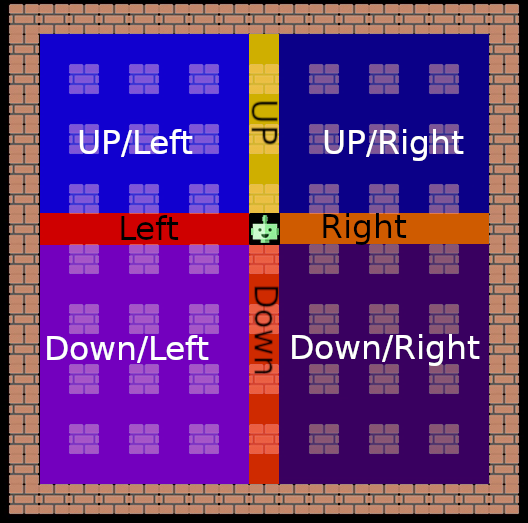
\includegraphics[width=\columnwidth]{Maze.png} % alternativ z.B. "width=6cm"
	\caption{Definition of the regions in the maze.}%
	\label{fig:Regions}%
\end{figure}

\subsubsection{Normalized potential rewards}

And in table \ref{table:S2} we show the regions regarding the second set, which make up the state. Each element, have the \textit{normalized potential rewards}(NPR) in each region, by mean of the $\omega_{R_{*}}$. And the weights $\omega_{R_{*}}$, are elements to measure  the potential reward to acquire, in all those eight regions described in figure \ref{fig:Regions}.

\begin{center}
\captionof{table}{How looks like the second array. Where the $\omega_{R_{*}}$ is the weight related to the NPR in each region.}
  \begin{tabular}{|c|}
\hline
Second array of the state: \\
\hline
$(\omega_{R_{U}},\omega_{R_{D}},\omega_{R_{L}},\omega_{R_{R}},\omega_{R_{UL}},\omega_{R_{DL}},\omega_{R_{DR}},\omega_{R_{UR}})$ \\
\hline
  \end{tabular}
  \label{table:S2}
\end{center}

Where:
\begin{equation}
    \omega_{R_*} \in [0,1]
\end{equation}


\subsubsection{Normalized potential danger}

The third set, is similar to the second one. 
Each element, takes into acount the \textit{ Normalized Potential Danger }(NPD) in each region. And each weights $\omega_{D_{*}}$, is a measure of the potential danger in all those eigth regions.

Similary to the table \ref{table:S2}, we show how looks like the \textbf{NPD} float array.
\begin{center}
\captionof{table}{How looks like the second array. Where the $\omega_{R_{D_*}}$ is the weight related to the \textbf{NPD} in each region.}
  \begin{tabular}{|c|}
\hline
How looks like the second array of the state: \\
\hline
$(\omega_{D_{U}},\omega_{D_{D}},\omega_{D_{L}},\omega_{D_{R}},\omega_{D_{UL}},\omega_{D_{DL}},\omega_{D_{DR}},\omega_{D_{UR}})$ \\
\hline
  \end{tabular}
  \label{table:S3}
\end{center}


Where:
\begin{equation}
    \omega_{R_*} \in [0,1]
\end{equation}

\subsubsection{Drop a bomb (DB): Feasibility and usefulness}

And to complete the state, we additionally add an array of two float values, regarding the situations where is feasible and useful to drop a bomb. The first value is a measure of the surrounding situation with the crates, and the second value is a measure of the proximity  of the opponents.

\begin{center}
\captionof{table}{How looks like the third array. Where the $\omega_{R_{D_Cr}}$ is the weight that measure the usefulness to get coins by blowing up crates, and $\omega_{R_{D_O}}$ the feasible of killing an opponent}
  \begin{tabular}{|c|}
\hline
How looks like the fourth array of the state: \\
\hline
$(\omega_{B_{Cr}},\omega_{B_{O}})$ \\
\hline
  \end{tabular}
  \label{table:S4}
\end{center}

Where:
\begin{equation}
    \omega_{B_*} \in [0,1]
\end{equation}

\subsubsection{Summary of state components}

In order to summarise the construct of the state, we describe the features selected. Which is made up of the four arrays shown in tables \ref{table:S1},\ref{table:S2},\ref{table:S3} and \ref{table:S4}:

\begin{table*}[t]
\centering
\captionof{table}{State summarized: Unsuccessfully attempt}
    \begin{tabular}{|l||c|c|c|r|}
     \hline
     \textbf{Abbreviation} & Description & Elements & Info & Type \\
     \hline
     \textbf{ACA}   &  Avalible cells & 4 & Directions & boolean \\
     \textbf{NPR}   &  Potential rewards & 8 & Regions & float  \\
     \textbf{NPD}   &  Potential danger & 8 & Regions & float  \\
     \textbf{DB}   &  Feasibility of throwing a bomb & 4 & Info crates and opponents & float  \\
     \hline
    \end{tabular}
    \label{table:S}
\end{table*}

\subsection{Second attempt: Simplifying the state}
\label{section:SimNRP}
With the aim to avoid correlated features, and achieve a functional version to complete the task 1 (\ref{section:Task1}). We simplify the NPR, in a binary version. 

The new NPR array is made up by four Booleans, where we calculate the nearest coin direction to operate the ACA with. 

\begin{figure}[t]% "t" = oben auf der Seite. Alternativ "b" f�r unten, "H" f�r direkt im Text
\centering	
	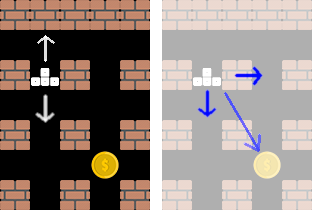
\includegraphics[width=\columnwidth]{NPR-1.png} % alternativ z.B. "width=6cm"
	\caption{Example of state formation, of ACA and NPR simplified: In right side the avalible moves is showed, then ACA is: (1100), and in the left side, the direction of probable reward (DPR), and is given by: (0101). 
	from operate with the $\land$ operator, we get the $NPR = (1100)\land (0101)=(0100)$ }%
	\label{fig:NPREx}%
\end{figure}

Using the \textit{AND} operator $\land$. We construct the \textit{NPR} array, a picted example is showed in figure \ref{fig:NPREx}. And in case of $ACA\land DPR=(0,0,0,0)$, we chose randomly the \textit{NPR} form the composed \textit{ACA} possibilities


\subsection{Task 1:}
\label{section:Task1}

{\it On a game board without any crates, collect a number of revealed coins as quickly as possible.
This task does not require dropping any bombs. The agent should learn how to navigate the
board effciently.}


For this task we use the state made up by the \textbf{ACA} array (see section \ref{section:ACA}) and the simplified \textbf{NRP} (see second \ref{section:SimNRP}). Summarised by the table \ref{table:Attemp2}.

\begin{table*}[!htbp]
\centering
\captionof{table}{State summarized}
    \begin{tabular}{|l||c|c|c|r|}
     \hline
     \textbf{Abbreviation} & Description & Elements & Info & Type \\
     \hline
     \textbf{ACA}   &  Avalible cells & 4 & Directions & Boolean \\
     \textbf{NPR simplified}   &  Nearest coin  & 4 & Directions & Boolean  \\
     \hline
    \end{tabular}
    \label{table:Attemp2}
\end{table*}

With the aim to kwon the learning evolution of the training, we calculate the total reward accumulated in all the training realization. At the begining of the training the amount of random actions predominate and the total reward accumulated start to decrease, later at the 150 episode, the agent will perform beter actions, and get positive rewards. Then, the total reward accumulated increase. See figure \ref{fig:TRewAccu}.

This behavior becomes clarified by mean of the figure \ref{fig:TRewAll}. Were shows, a convergence tendence after episode $400$. Up to get a maximal rewarded performed of $828$ (green)

For this task, the agent must to learn two diferent skills. The fisrt one, is the skill to avoid the invalid actions, and the second one is to chose effciently the path to the coins. 
In order to measure those skills, we show \cite{paperDQL}


\begin{figure}[t]% "t" = oben auf der Seite. Alternativ "b" f�r unten, "H" f�r direkt im Text
	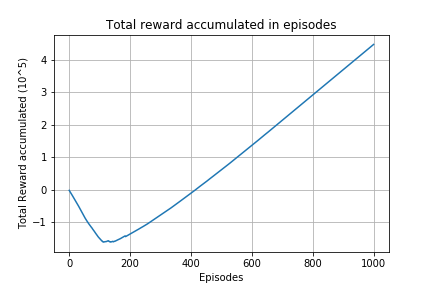
\includegraphics[width=\columnwidth]{TRewAccu.png} % alternativ z.B. "width=6cm"
	\caption{Total reward accumulated in episodes}%
	\label{fig:TRewAccu}%
\end{figure}

\begin{figure}[t]% "t" = oben auf der Seite. Alternativ "b" f�r unten, "H" f�r direkt im Text
	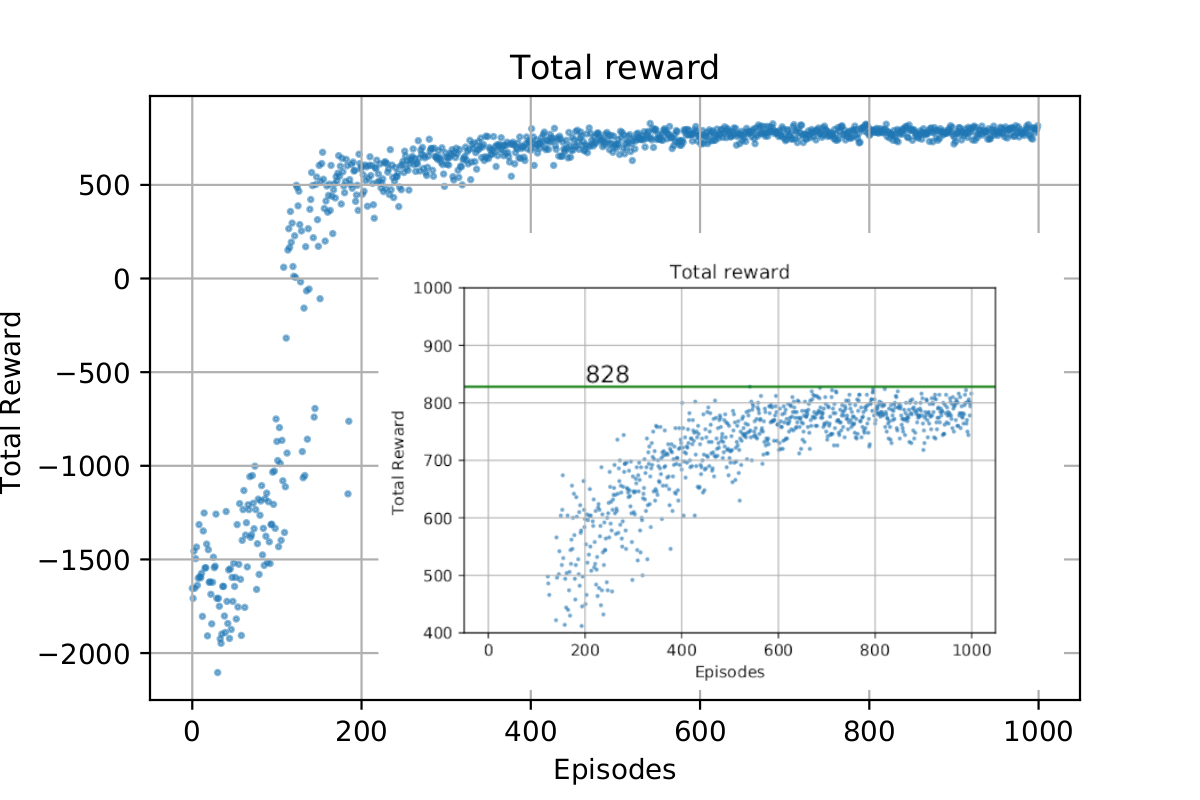
\includegraphics[width=\columnwidth]{TRewAll.png} % alternativ z.B. "width=6cm"
	\caption{Total reward in episodes. Plot inside: detailed behavior (in order to show the total reward tendence))}%
	\label{fig:TRewAll}%
\end{figure}

\begin{figure}[t]% "t" = oben auf der Seite. Alternativ "b" f�r unten, "H" f�r direkt im Text
	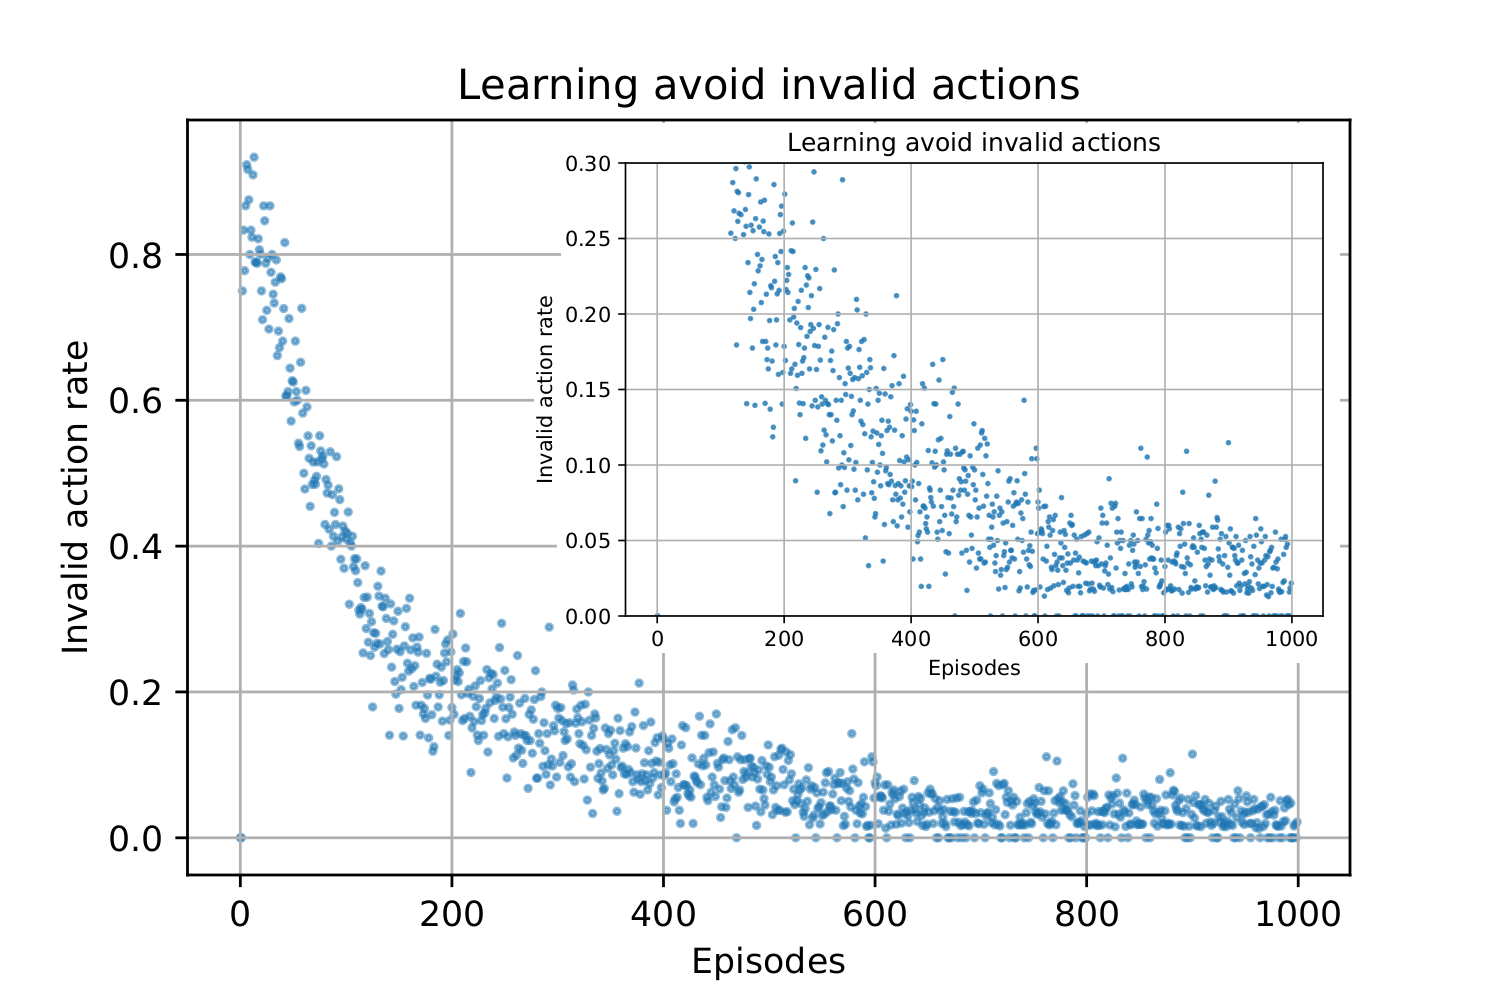
\includegraphics[width=\columnwidth]{Meassure1Coins.png} % alternativ z.B. "width=6cm"
	\caption{Meassuring the learning to avoid invalid actions. Plot inside: detailed behavior (in order to show the xtendence))}%
	\label{fig:M1Coins}%
\end{figure}


\begin{figure}[t]% "t" = oben auf der Seite. Alternativ "b" f�r unten, "H" f�r direkt im Text
	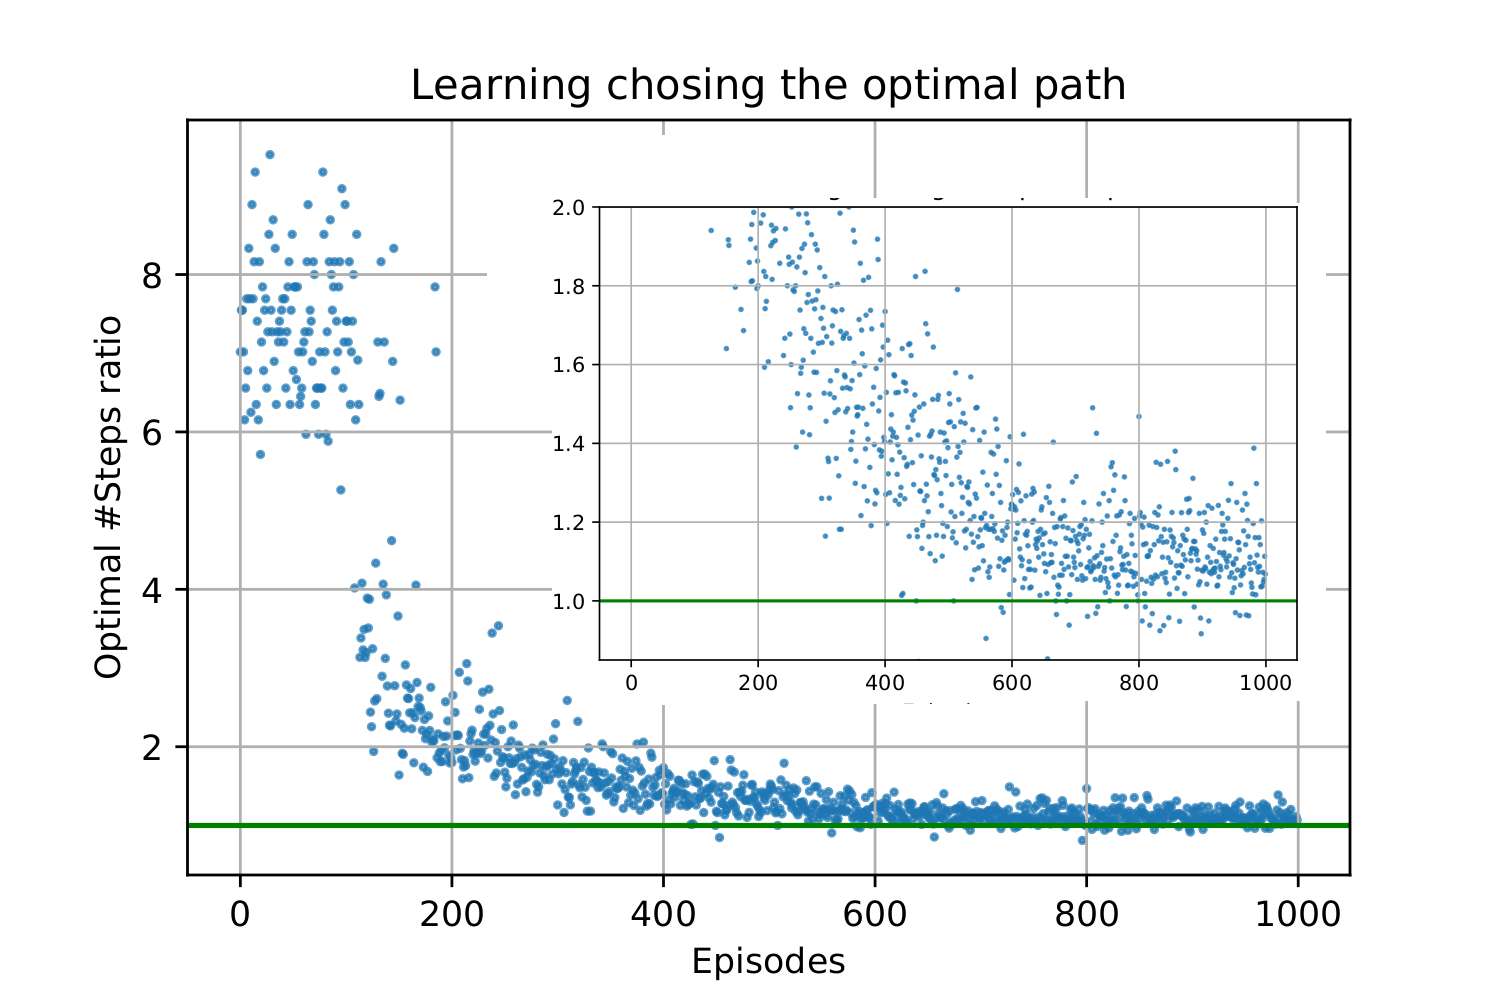
\includegraphics[width=\columnwidth]{Meassure2Coins.png} % alternativ z.B. "width=6cm"
	\caption{Meassuring the learning find the optimal path to get the coins. Plot inside: detailed behavior (in order to show the tendence))}%
	\label{fig:M1Coins}%
\end{figure}








